\documentclass[12pt]{kiarticle}
\graphicspath{{pictures/}}
\DeclareGraphicsExtensions{.pdf,.png,.jpg,.eps}
%%%
\pagestyle{fancy}
\fancyhf{}
%\renewcommand{\headrulewidth}{ 0.1mm }
\renewcommand{\footrulewidth}{ .0em }
\fancyfoot[C]{\texttt{\textemdash~\thepage~\textemdash}}
\fancyhead[L]{Лабораторная работа № 4.5.2 \hfil}
\fancyhead[R]{\hfil Иванов Кирилл, 625 группа }
\usepackage{multirow} % Слияние строк в таблице
\newcommand
{\un}[1]
{\ensuremath{\text{#1}}}
\newcommand{\eds}{\ensuremath{ \mathscr{E}}}
\usepackage{tikz}
%%% Работа с таблицами
\usepackage{array,tabularx,tabulary,booktabs} % Дополнительная работа с таблицами
\usepackage{longtable}  % Длинные таблицы
\usepackage{multirow} % Слияние строк в таблице

\begin{document}
	
	\begin{titlepage}
	\begin{center}
		\large 	Московский физико-технический институт \\
		(государственный университет) \\
		Факультет общей и прикладной физики \\
		\vspace{0.2cm}
		
		\vspace{4.5cm}
		Лабораторная работа № 4.5.2 \\ \vspace{0.2cm}
		\large (Общая физика: оптика) \\ \vspace{0.2cm}
		\LARGE \textbf{Интерференция лазерного излучения}
	\end{center}
	\vspace{2.3cm} \large
	
	\begin{center}
		Работу выполнил: \\
		Иванов Кирилл,
		625 группа
		\vspace{10mm}		
		
	\end{center}
	
	\begin{center} \vspace{60mm}
		г. Долгопрудный \\
		2018 год
	\end{center}
\end{titlepage}
	
	\paragraph*{Цель работы:} исследование видности интерференционной картины излучения гелий-неонового лазера и определение длины когерентности излучения.
	
	\paragraph*{Оборудование:}  $Не-Nе$-лазер, интерферометр Майкельсона с подвижным зеркалом, фотодиод с усилителем, осциллограф, поляроид, линейка.
	
	\section{Теоретическое введение}
	
	Важный параметр интерференционной картины --- ее видимость:
	
	\begin{equation}\label{V0}
	V = \dfrac{I_{max} - I_{min}}{I_{max} + I_{min}}
	\end{equation}
	
	Удобно представлять видимость в виде произведения функций различных параметров установки/системы:
	
	\begin{equation}\label{VVV}
	V = V_1 V_2 V_3
	\end{equation}
	
	Рассмотрим эти функции подробнее. Первая из них отвечает за отношение интенсивностей интерферирующих волн:
	
	\begin{equation}\label{V1}
	V_1 = \dfrac{2\sqrt{\delta}}{1 + \delta}, \quad \delta = \dfrac{B_m^2}{A_m^2}
	\end{equation}
	
	\begin{wrapfigure}{l}{0.35\linewidth} 
		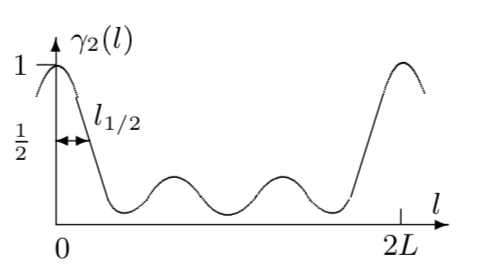
\includegraphics[width=\linewidth]{v2}
		\caption{Качественный график $ V_2 $}
		\label{V2graf}
	\end{wrapfigure}
	
	
	Здесь $ A_m, B_m $ --- амплитуды волн. Вторая функция учитывает влияние разности хода и спектрального состава волн:
	
	\begin{equation}\label{}
	\gamma_2 = \dfrac{\sum\limits_n A_n^2 \cos{\dfrac{2\pi \Delta \nu n l}{c}}}{\sum\limits_n A_n^2} \sim e^{-(\pi \Delta F l /c^2)}
	\end{equation}
	
	
	Здесь $ l $ --- разность хода, $ \Delta\nu $ --- спектральный состав излучения, $ A_n^2 $ --- интенсивность мод. Оценка приведена из перехода к непрерывному пределу. Последняя функция --- зависимость от угла поляризации $ \alpha $:
	
	\begin{equation}\label{}
	V_3 = |\cos{\alpha}|
	\end{equation}
	
	\section{Экспериментальная установка}
	
	\subsection{Описание установки}
	
	Для получения интерференционной картины используется интерферометр Майкельсона, смонтированный на вертикально стоящей массивной металлической плите. Схема установки приведена на рисунке.
	
\begin{figure}[h!]
		\centering
		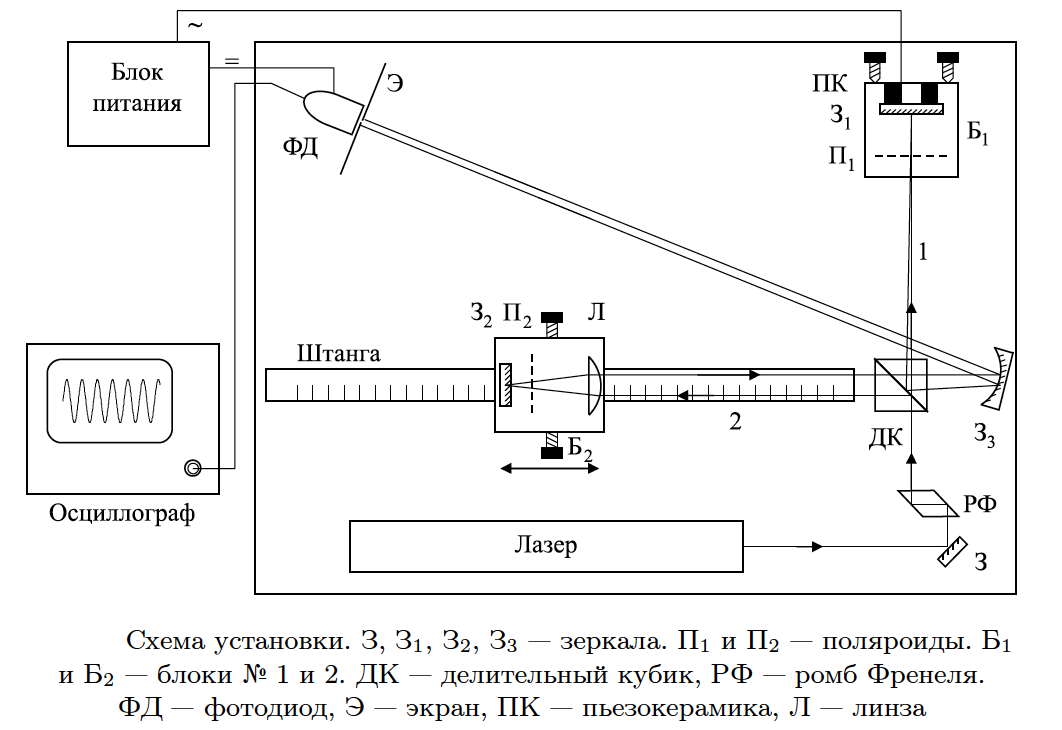
\includegraphics[width=\linewidth]{lab.png}
%		\caption{Экспериментальная установка}
		\label{lab}
\end{figure}

Источником света служит гелий-неоновый лазер (средняя длина
волны $ \lambda_0 = 632,8 $ нм). Пучок лазерного излучения отражается от зеркала З и проходит призму полного внутреннего отражения РФ (ромб Френеля), которая превращает линейную поляризацию излучения в круговую. Если в установке используется лазер, излучающий неполяризованный свет, то ромб Френеля не нужен, но он и не мешает выполнению
работы. Далее лазерное излучение делится диагональной плоскостью
делительного кубика ДК на два пучка.

Пучок 1 проходит поляроид $ П_1, $ отражается под небольшим углом
от зеркала $ З_1 $, снова проходит поляроид $ П_1 $ и, частично отражаясь от
диагональной плоскости делительного кубика, выходит из интерферометра, попадает на зеркало $ З_3 $ и далее на фотодиод ФД. Зеркало $ З_1 $
наклеено на пьезокерамику ПК, которая может осуществлять малые колебания зеркала вдоль направления распространения падающего пуч-
ка. Поляроид и зеркало с пьезокерамикой собраны в единый блок $ Б_1 $,
который крепится к вертикально стоящей плите. В блоке $ Б_1 $ имеются
юстировочные винты, которые позволяют регулировать угол наклона
зеркала $ З_1 $. В установке предусмотрена возможность вращения поляро-
ида $ П_1 $. Угол поворота отсчитывается по шкале, нанесённой на оправу
поляроида.
Пучок 2 проходит линзу Л, поляроид $ П_2 $, отражается от зеркала $ З_2 $,
снова проходит поляроид $ П_2 $, линзу Л и делительный кубик, выходит из
интерферометра, попадает на зеркало $ З_3 $ и далее на фотодиод ФД. Та-
ким образом, от зеркала $ З_3 $ под небольшим углом друг к другу идут на
фотодиод два пучка, прошедшие разные плечи интерферометра. Меж-
ду ними происходит интерференция и образуются интерференционные
полосы. Линза Л, поляроид $ П_2 $ и зеркало $ З_2 $ собраны в единый блок $ Б_2 $.

Зеркало $ З_2 $ установлено в фокальной плоскости линзы Л. Это сделано
для того, чтобы падающий и выходящий из блока $ Б_2 $ пучки всегда были
параллельны друг другу. Блок $ Б_2 $ может перемещаться вдоль пучка 2
по штанге, жёстко связанной с плитой интерферометра. Длина штанги
90 см. В установке предусмотрена возможность небольшого поперечно-
го перемещения блока $ Б_2 $, что позволяет регулировать расстояние меж-
ду падающим и выходящим из блока пучками. При измерениях блок
Б2 крепится к штанге при помощи двух винтов. Вдоль штанги нанесены деления через один сантиметр. При перемещении блока $ Б_2 $ вдоль
штанги на величину $ x_1 $ геометрическая разность хода между пучками
1 и 2 изменяется на величину $ l = 2x_1 $.

Сферическое зеркало $ З_3 $ с небольшим фокусным расстоянием увеличивает картину интерференционных полос и позволяет наблюдать её
на экране Э, расположенном в плоскости входного окна фотодиода.
Свет попадает на фотодиод ФД через узкую щель в центре экрана.
Щель ориентируется параллельно интерференционным полосам. Ширина щели меньше расстояния между полосами. Сигнал фотодиода усиливается и подаётся на вход осциллографа. Для питания усилителя
сигнала фотодиода и управления пьезокерамикой используется блок
питания БП.

На пьезокерамику подаётся напряжение с частотой 50 Гц. При этом
её длина изменяется с частотой 100 Гц. Величина удлинения зависит от
приложенного напряжения и регулируется ручкой "<Качание"> на блоке
питания. Обычно удлинение составляет несколько длин волн света. На
эту величину перемещается вдоль пучка 1 зеркало $ З_1 $. Интерференционная картина смещается на ширину полосы (одно колебание на экране осциллографа), если зеркало $ З_1 $ смещается на $ \lambda_0 /2 \sim 0,3 $ мкм. При
измерениях через входную щель фотодиода последовательно проходит
несколько полос интерференционной картины, а на экране осциллографа наблюдаются колебания с изменяющимся периодом.

\subsection{Методика измерения}

\begin{wrapfigure}{l}{0.35\linewidth} 
	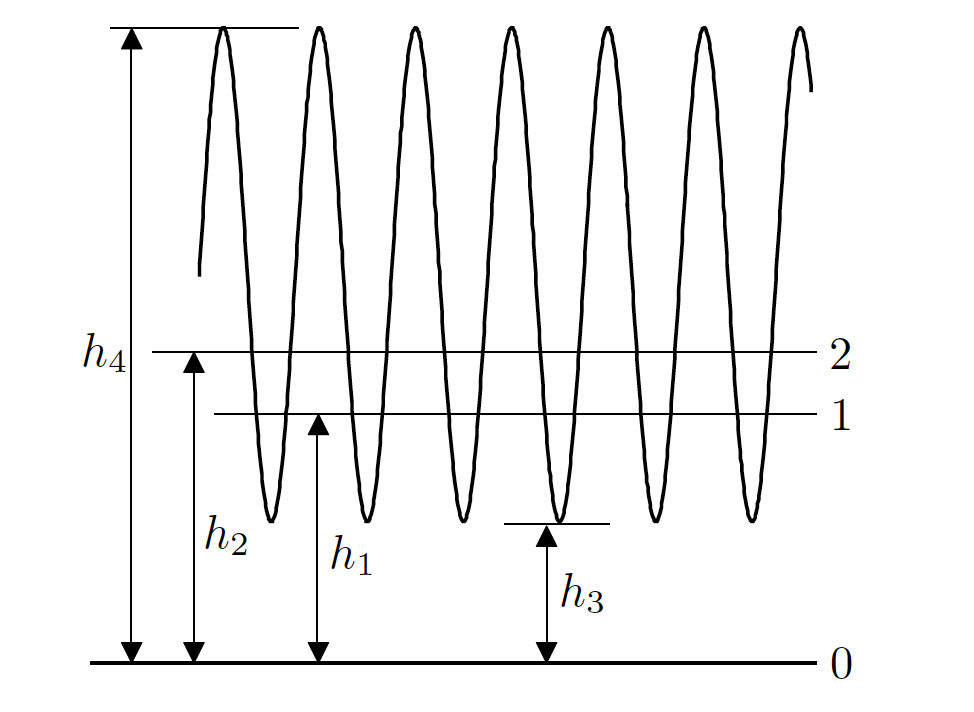
\includegraphics[width=\linewidth]{os}
	\caption{Сигнал фотодиода на осциллографе}
	\label{}
\end{wrapfigure}

	Осциллограф мы используем для нахождения следующих вели-
чин: фоновой засветки (линия 0 --- перекрыты оба пучка 1 и 2); интенсивность света каждого из пучков (линии 1 или 2 --- перекрыт пучок
2 или 1); максимума и минимума интенсивности интерференционной
картины (открыты оба пучка). При этом параметр $ \delta $ из \eqref{V1},  определяется отношением

\begin{equation}\label{delta}
\delta = \dfrac{h_1}{h_2}
\end{equation}

Понятно, что из физического смысла, наша видимость рассчитывается очевидным образом, согласно формуле \eqref{V0}, так:

\begin{equation}\label{V}
V = \dfrac{h_4 - h_3}{h_4 + h_3}
\end{equation}

Отсюда, используя \eqref{VVV}, мы можем получить наши функции из \eqref{V}, фиксируя одну из них (т.е. беря равной единице). Так, при $ \alpha = 0 \te V_3 = 1 $, 

\begin{equation}\label{V2}
V_2 (l) = \dfrac{V}{V_1} = \dfrac{h_4 - h_3}{h_4 + h_3} \x \dfrac{h_2}{h_1}
\end{equation}

А приняв разность хода $ l = 0 \te V_2 = 0 $, можно найти 

\begin{equation}\label{V_3}
V_3(\alpha) = \dfrac{V}{V_1} = \dfrac{h_4 - h_3}{h_4 + h_3} \x \dfrac{h_2}{h_1}
\end{equation}

\section{Ход работы}

\subsection{Изучение поляризации}

Поворотами поляризатора $ П_1 $ убедимся, что свет от лазера --- поляризованный. Настроив поляроид на минимальную видимость и введя дополнительный поляроид, мы вновь получаем интерференционную картину при его поворотах. Так как картина изменятся линейно, получаем, что \textbf{поляризация --- линейная}.

\subsection{Измерение коэффициента видимости от угла}

Исследуем зависимость видности интерференционной картины от угла
$ \beta $ поворота поляроида $ П_1 $ при нулевой разности хода ($ V_2 = 1 $). Для этого измерим величины $ h_1, h_2, h_3 \; и \; h_4 $ на экране осциллографа. Результаты занесем в таблицу.


	
	\end{document}